\documentclass[10pt,aspectratio=169]{beamer}

\usetheme[progressbar=foot]{metropolis}
\AtBeginSection{}

\usepackage{appendixnumberbeamer}
\usepackage{booktabs}
\usepackage[scale=2]{ccicons}
\usepackage{tabularx}
\usepackage{tikz}
\usetikzlibrary{arrows.meta,positioning,shapes.geometric,fit,calc}
\usepackage{xspace}
\newcommand{\themename}{\textbf{\textsc{metropolis}}\xspace}
\usepackage{comment}
\usepackage{caption}
\usepackage[
  backend=biber,
  style=authoryear
]{biblatex}

\setbeamertemplate{bibliography item}{}
\addbibresource{bibliography.bib}

\usepackage{graphicx}
\usepackage{siunitx}



%................................................................................
% COLORS

\definecolor{ukudlaBlue}{RGB}{41, 60, 135}
\definecolor{ukudlaLightBlue}{RGB}{212, 216, 231}
\definecolor{ukudlaRed}{RGB}{164, 28, 34}
\definecolor{ukudlaLightRed}{RGB}{236, 209, 210}
\definecolor{ukudlaGreen}{RGB}{59, 139, 71}
\definecolor{ukudlaLightGreen}{RGB}{215, 231, 218}
\definecolor{ukudlaYellow}{RGB}{239, 198, 44}
\definecolor{ukudlaLightYellow}{RGB}{251, 243, 212}
\definecolor{white}{RGB}{255, 255, 255}
\definecolor{black}{RGB}{0, 0, 0}

\setbeamercolor{palette primary}{fg=white, bg=ukudlaGreen}
\setbeamercolor{progress bar}{fg=ukudlaRed, bg=ukudlaYellow}
\setbeamercolor{title separator}{fg=ukudlaRed, bg=ukudlaYellow}
\setbeamercolor{progress bar in head/foot}{fg=ukudlaRed, bg=ukudlaYellow}
\setbeamercolor{progress bar in section page}{fg=ukudlaRed, bg=ukudlaYellow}
\setbeamercolor{background canvas}{bg=white}
\setbeamercolor{block body}{bg=ukudlaLightGreen,fg=black}



%................................................................................
% PRESENTATION INFORMATION

\title{UKUDLA Data Science Certificate}
\subtitle{Predictive Analysis}
\author{Markus Mößler}
\institute{University of Hohenheim}



%................................................................................
% CUSTOM FOOTER

\makeatletter
\setbeamertemplate{progress bar in head/foot}{%
  \tikzset{metropolis@progressbar@foreground/.style={fill=ukudlaGreen}}%
  \tikzset{metropolis@progressbar@background/.style={fill=ukudlaLightGreen}}%

  \begin{tikzpicture}[overlay, x=\paperwidth, y=1cm]
    \fill[metropolis@progressbar@background]
      (0,0) rectangle (1,0.10);
    \fill[metropolis@progressbar@foreground]
      (0,0) rectangle
      ({\insertframenumber/\inserttotalframenumber},0.10);
    \node[anchor=south west, yshift=0.25cm, xshift=0.2cm]
      at (0,0)
      {\includegraphics[height=0.75cm]{./logos/UKUDLA_logo_03_white_bg.pdf}};
    % current section
    \ifnum\value{section}>0
      \node[
        anchor=south east,
        yshift=0.22cm,
        xshift=-0.60cm,
        fill=ukudlaLightGreen,
        rounded corners=2pt,
        inner xsep=6pt,
        inner ysep=3pt,
        font=\scriptsize\bfseries,
        text=ukudlaRed
      ] at (1,0) {
        \insertsectionhead
      };
    \fi

  \end{tikzpicture}%
}
\makeatother



%................................................................................
% CUSTOM TITLE PAGE

\makeatletter
\setbeamertemplate{title page}{
  \begin{beamercolorbox}[sep=8pt, center, wd=\paperwidth, ht=0.5\paperheight]{title page top}
    \begin{minipage}[c]{1.00\textwidth}
      \raggedleft
      \includegraphics[height=1.00cm]{./logos/ukudla_universities.pdf}
      \vspace*{0.2cm}
    \end{minipage}
    \begin{beamercolorbox}[wd=0.9\paperwidth, sep=12pt, left]{top box}
      {\usebeamerfont{title}\usebeamercolor[fg]{title}\inserttitle\par}
      \vskip0.1cm
      {\usebeamerfont{subtitle}\usebeamercolor[fg]{subtitle}\insertsubtitle\par}
    \end{beamercolorbox}
  \end{beamercolorbox}
  \begin{beamercolorbox}[sep=8pt, center, wd=\paperwidth, ht=0.5\paperheight]{title page bottom}
    \begin{beamercolorbox}[wd=0.9\paperwidth, sep=12pt, left]{bottom box}
      \hbox{%
        \hspace*{1em}
        \begin{minipage}[c]{0.40\textwidth}
          \vskip1.0cm
          {\usebeamerfont{author}\usebeamercolor[fg]{author}\insertauthor\par}
          \vskip0.1cm
          {\usebeamerfont{institute}\usebeamercolor[fg]{institute}\insertinstitute\par}
        \end{minipage}%
        \hspace*{1.5cm}
        \begin{minipage}[c]{1.00\textwidth}
          \includegraphics[height=2.0cm]{./logos/UKUDLA_logo_05.pdf}
        \end{minipage}%
      }
    \end{beamercolorbox}
    \begin{minipage}[r]{1.00\textwidth}
      \centering
      \includegraphics[width=1.00\textwidth]{./logos/ukudla_sponsors.pdf}
    \end{minipage}
  \end{beamercolorbox}
}
\makeatother

\setbeamercolor{title page top}{bg=white}
\setbeamercolor{top box}{bg=ukudlaGreen}
\setbeamercolor{title page bottom}{bg=white}
\setbeamercolor{bottom box}{bg=ukudlaLightGreen}
\setbeamercolor{title}{fg=white}
\setbeamercolor{subtitle}{fg=white}
\setbeamercolor{author}{fg=black}
\setbeamercolor{institute}{fg=black}
\setbeamercolor{date}{fg=black}



%................................................................................
% DOCUMENT

\begin{document}

\maketitle

%--------------------------------------------------
{
\setbeamertemplate{frame numbering}[none]

\begin{frame}[noframenumbering]{Table of contents}

  \small
  \setbeamertemplate{section in toc}[sections numbered]
  \tableofcontents[hideallsubsections]

\end{frame}
}
%--------------------------------------------------



\section{Motivation}


%--------------------------------------------------
% CONTENT SLIDE 1/10
\begin{frame}{Explanation and prediction answer different questions}

\small

\begin{columns}[T]

\column{0.47\textwidth}

\textbf{Explanatory objective}

\begin{itemize}
  \item What causal relationship is of interest?
  \item Which assumptions identify the effect?
  \item How should a coefficient be interpreted?
  \item Which alternative explanations remain?
\end{itemize}

\column{0.47\textwidth}

\textbf{Predictive objective}

\begin{itemize}
  \item What outcome must be predicted?
  \item Which information is available at prediction time?
  \item How accurate are predictions on unseen observations?
  \item Where and when does performance fail?
\end{itemize}

\end{columns}

\vspace{0.35cm}

\begin{beamercolorbox}[rounded=true,sep=8pt]{block body}
A variable can improve prediction without causing the outcome. A causally meaningful model can still predict poorly when the future differs from its training data.
\end{beamercolorbox}

\vspace{0.15cm}

\centering
\textcolor{ukudlaRed}{Choose the objective before choosing the model or metric.}

\end{frame}
%--------------------------------------------------


%--------------------------------------------------
% CONTENT SLIDE 2/10
\begin{frame}{Evaluation must reproduce the intended use}

\small

\begin{center}
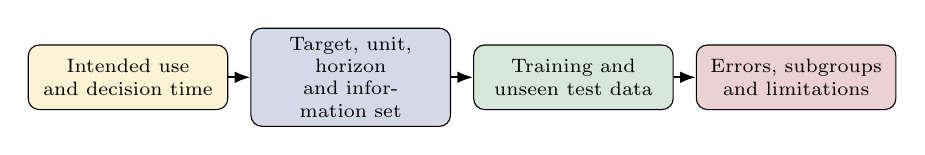
\begin{tikzpicture}[
  node distance=0.28cm,
  box/.style={draw, rounded corners, align=center, minimum height=0.82cm,
              text width=2.30cm, font=\scriptsize},
  arrow/.style={-{Latex[length=2mm]}, thick}
]
\node[box, fill=ukudlaLightYellow] (use) {Intended use\\and decision time};
\node[box, fill=ukudlaLightBlue, right=of use] (task) {Target, unit, horizon\\and information set};
\node[box, fill=ukudlaLightGreen, right=of task] (split) {Training and\\unseen test data};
\node[box, fill=ukudlaLightRed, right=of split] (evaluate) {Errors, subgroups\\and limitations};
\draw[arrow] (use) -- (task);
\draw[arrow] (task) -- (split);
\draw[arrow] (split) -- (evaluate);
\end{tikzpicture}
\end{center}

\vspace{0.35cm}

\begin{itemize}
  \item Training performance measures how well a model fits data it has already seen.
  \item Test performance estimates generalization only when the test mimics future use.
  \item Time-dependent data usually require earlier training and later testing.
  \item Any information unavailable at prediction time creates leakage.
\end{itemize}

\vspace{0.20cm}

\centering
\textcolor{ukudlaRed}{A convenient random split can answer the wrong performance question.}

\end{frame}
%--------------------------------------------------



\section{Concepts}


%--------------------------------------------------
% CONTENT SLIDE 3/10
\begin{frame}{Define a prediction contract}

\small

\begin{columns}[T]

\column{0.31\textwidth}

\textbf{Prediction target}

\begin{itemize}
  \item outcome and unit;
  \item target population;
  \item prediction horizon; and
  \item scale and required output.
\end{itemize}

\column{0.31\textwidth}

\textbf{Information set}

\begin{itemize}
  \item prediction time;
  \item variables available then;
  \item data latency and revisions; and
  \item allowed history.
\end{itemize}

\column{0.33\textwidth}

\textbf{Evaluation contract}

\begin{itemize}
  \item split strategy;
  \item baselines and candidates;
  \item metrics and subgroups; and
  \item intended and excluded uses.
\end{itemize}

\end{columns}

\vspace{0.35cm}

\begin{beamercolorbox}[rounded=true,sep=8pt]{block body}
Predicting before sampling, during an experiment, or after data collection are different tasks because their horizons and available information differ.
\end{beamercolorbox}

\end{frame}
%--------------------------------------------------


%--------------------------------------------------
% CONTENT SLIDE 4/10
\begin{frame}{Training, validation and testing have distinct roles}

\small

\begin{center}
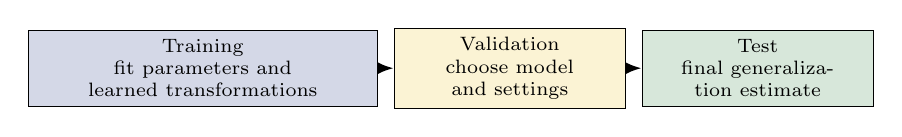
\begin{tikzpicture}[
  node distance=0.20cm,
  period/.style={draw, minimum height=0.85cm, align=center, font=\scriptsize},
  arrow/.style={-{Latex[length=2mm]}, thick}
]
\node[period, fill=ukudlaLightBlue, text width=4.20cm] (train) {Training\\fit parameters and learned transformations};
\node[period, fill=ukudlaLightYellow, text width=2.70cm, right=of train] (validation) {Validation\\choose model and settings};
\node[period, fill=ukudlaLightGreen, text width=2.70cm, right=of validation] (test) {Test\\final generalization estimate};
\draw[arrow] (train) -- (validation);
\draw[arrow] (validation) -- (test);
\end{tikzpicture}
\end{center}

\vspace{0.30cm}

\begin{itemize}
  \item Fit imputation, scaling, feature selection and model parameters on training data only.
  \item Use validation or resampling to compare alternatives without consuming the test set.
  \item Inspect the test set once the workflow is fixed; repeated tuning turns it into validation data.
  \item Preserve groups and temporal order when they define the deployment problem.
\end{itemize}

\vspace{0.20cm}

\centering
\textcolor{ukudlaRed}{The test set protects an honest question only while it remains unseen.}

\end{frame}
%--------------------------------------------------


%--------------------------------------------------
% CONTENT SLIDE 5/10
\begin{frame}{Leakage makes performance look better than use}

\small

\begin{columns}[T]

\column{0.47\textwidth}

\textbf{Common leakage routes}

\begin{itemize}
  \item future outcomes or revised future records;
  \item preprocessing learned from all observations;
  \item selecting variables after test inspection;
  \item duplicate or related units across splits;
  \item predictors measured after the prediction time.
\end{itemize}

\column{0.47\textwidth}

\textbf{Prevent leakage through design}

\begin{itemize}
  \item timestamp every input by availability;
  \item split before learned preprocessing;
  \item fit the complete recipe on training data;
  \item preserve group and time boundaries;
  \item document every test-set interaction.
\end{itemize}

\end{columns}

\vspace{0.35cm}

\begin{beamercolorbox}[rounded=true,sep=8pt]{block body}
A measurement can be a predictor only if it is available when the intended prediction is made. Otherwise the task and its claimed horizon must be redefined.
\end{beamercolorbox}

\end{frame}
%--------------------------------------------------


%--------------------------------------------------
% CONTENT SLIDE 6/10
\begin{frame}{Baselines define the minimum useful performance}

\small

\begin{tabularx}{\textwidth}{@{}p{0.25\textwidth}X X@{}}
\toprule
\textbf{Candidate} & \textbf{Prediction rule} & \textbf{What it tests} \\
\midrule
Historical mean & Predict one training-period average & Can any structure beat a constant? \\
Group mean & Predict each relevant group's training average & Is group identity enough? \\
Linear trend & Extrapolate a training-period time trend & Does temporal structure help? \\
Group + trend & Combine group levels and time & Does structured regression generalize? \\
Added predictors & Use variables available at prediction time & Does extra complexity earn its cost? \\
\bottomrule
\end{tabularx}

\vspace{0.30cm}

\begin{itemize}
  \item A baseline must follow the same split and information rules as every candidate.
  \item More complex models must improve relevant unseen-data performance, not only training fit.
  \item Simplicity, stability, computation and interpretability remain deployment considerations.
\end{itemize}

\end{frame}
%--------------------------------------------------


%--------------------------------------------------
\section{Application}
% CONTENT SLIDE 7/10

\begin{frame}{Metrics summarize errors---and hide structure}

\small

\begin{columns}[T]

\column{0.47\textwidth}

\textbf{Prediction error}

\[
e_i = y_i - \hat{y}_i
\]

\[
\mathrm{MAE}=\frac{1}{n}\sum_{i=1}^{n}|e_i|
\]

\[
\mathrm{RMSE}=\sqrt{\frac{1}{n}\sum_{i=1}^{n}e_i^2}
\]

\column{0.47\textwidth}

\textbf{Interpret with context}

\begin{itemize}
  \item MAE weights absolute errors linearly;
  \item RMSE emphasizes larger errors;
  \item units follow the modeled outcome scale;
  \item averages can hide group, site or period failures;
  \item uncertainty grows with small test sets.
\end{itemize}

\end{columns}

\vspace{0.25cm}

\begin{beamercolorbox}[rounded=true,sep=8pt]{block body}
Generalization depends on similarity between evaluation and use. Batch effects, site differences, temporal shifts and new populations can make test performance optimistic.
\end{beamercolorbox}

\end{frame}
%--------------------------------------------------



%--------------------------------------------------
% CONTENT SLIDE 8/10
\begin{frame}{Define a prediction task before model fitting}

\small

\begin{columns}[T]

\column{0.47\textwidth}

\textbf{Prediction contract}

\begin{itemize}
  \item target, unit and prediction scale;
  \item target population and observation grain;
  \item prediction time and horizon;
  \item development and evaluation periods;
  \item information available at prediction time.
\end{itemize}

\column{0.47\textwidth}

\textbf{Boundary}

\begin{itemize}
  \item test outcomes remain unseen during fitting;
  \item the evaluation represents the intended population;
  \item temporal prediction may require extrapolation;
  \item unavailable future information is excluded;
  \item supported and excluded uses are documented.
\end{itemize}

\end{columns}

\vspace{0.25cm}

\centering
\textcolor{ukudlaRed}{The split must ask whether patterns learned from available data transfer to the intended use.}

\end{frame}
%--------------------------------------------------


%--------------------------------------------------
% CONTENT SLIDE 9/10
\begin{frame}{Fit on development data and predict held-out observations}

\small

\begin{center}
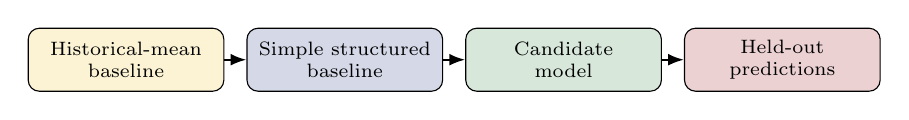
\begin{tikzpicture}[
  node distance=0.28cm,
  box/.style={draw, rounded corners, align=center, minimum height=0.80cm,
              text width=2.25cm, font=\scriptsize},
  arrow/.style={-{Latex[length=2mm]}, thick}
]
\node[box, fill=ukudlaLightYellow] (mean) {Historical-mean\\baseline};
\node[box, fill=ukudlaLightBlue, right=of mean] (trend) {Simple structured\\baseline};
\node[box, fill=ukudlaLightGreen, right=of trend] (country) {Candidate\\model};
\node[box, fill=ukudlaLightRed, right=of country] (predictions) {Held-out\\predictions};
\draw[arrow] (mean) -- (trend);
\draw[arrow] (trend) -- (country);
\draw[arrow] (country) -- (predictions);
\end{tikzpicture}
\end{center}

\vspace{0.30cm}

\begin{itemize}
  \item Learn every transformation and parameter from development data only.
  \item Generate one prediction from each candidate for every held-out observation.
  \item Preserve observed outcomes only for evaluation after prediction.
  \item Save model objects, split definitions and row-level predictions reproducibly.
  \item Add predictors only when their availability matches the prediction time.
\end{itemize}

\end{frame}
%--------------------------------------------------


%--------------------------------------------------
\section{Key Message}
% CONTENT SLIDE 10/10

\begin{frame}{Key message: evaluate the complete predictive workflow}

\small

\begin{columns}[T]

\column{0.47\textwidth}

\textbf{Evidence to deliver}

\begin{itemize}
  \item prediction contract and split manifest;
  \item row-level held-out predictions;
  \item MAE and RMSE overall and by relevant group;
  \item error plots over groups and time;
  \item comparison with every baseline; and
  \item reproducible model artifacts and report.
\end{itemize}

\column{0.47\textwidth}

\textbf{Limitations to state}

\begin{itemize}
  \item small test sets provide limited evidence;
  \item performance can differ across groups;
  \item future distribution shifts remain possible;
  \item log-scale errors need outcome-scale context;
  \item predictive accuracy does not imply causality.
\end{itemize}

\end{columns}

\vspace{0.30cm}

\begin{beamercolorbox}[rounded=true,sep=8pt]{block body}
A predictive model is useful only for a stated task when it improves on relevant baselines, survives realistic unseen-data evaluation and remains reproducible at the point of use.
\end{beamercolorbox}

\vspace{0.15cm}

\centering
\textcolor{ukudlaRed}{Report where the model works, where it fails and where the evidence ends.}

\end{frame}
%--------------------------------------------------


%--------------------------------------------------
\begin{frame}[plain,noframenumbering]{Supported by}

  South African government and the National Research Foundation

  \begin{flushleft}
    \includegraphics[trim=0cm 0cm 0cm 0cm, clip, width=0.50\textwidth]{./logos/ukudla_south_african_sponsors.pdf}
  \end{flushleft}

  German government and the German Academic Exchange Service

  \begin{flushleft}
    \includegraphics[trim=0cm 0cm 0cm 0cm, clip, width=1.00\textwidth]{./logos/ukudla_german_sponsors.pdf}
  \end{flushleft}

\end{frame}
%--------------------------------------------------

\end{document}
